% Options for packages loaded elsewhere
% Options for packages loaded elsewhere
\PassOptionsToPackage{unicode}{hyperref}
\PassOptionsToPackage{hyphens}{url}
\PassOptionsToPackage{dvipsnames,svgnames,x11names}{xcolor}
%
\documentclass[
  letterpaper,
  DIV=11,
  numbers=noendperiod]{scrreprt}
\usepackage{xcolor}
\usepackage{amsmath,amssymb}
\setcounter{secnumdepth}{5}
\usepackage{iftex}
\ifPDFTeX
  \usepackage[T1]{fontenc}
  \usepackage[utf8]{inputenc}
  \usepackage{textcomp} % provide euro and other symbols
\else % if luatex or xetex
  \usepackage{unicode-math} % this also loads fontspec
  \defaultfontfeatures{Scale=MatchLowercase}
  \defaultfontfeatures[\rmfamily]{Ligatures=TeX,Scale=1}
\fi
\usepackage{lmodern}
\ifPDFTeX\else
  % xetex/luatex font selection
\fi
% Use upquote if available, for straight quotes in verbatim environments
\IfFileExists{upquote.sty}{\usepackage{upquote}}{}
\IfFileExists{microtype.sty}{% use microtype if available
  \usepackage[]{microtype}
  \UseMicrotypeSet[protrusion]{basicmath} % disable protrusion for tt fonts
}{}
\makeatletter
\@ifundefined{KOMAClassName}{% if non-KOMA class
  \IfFileExists{parskip.sty}{%
    \usepackage{parskip}
  }{% else
    \setlength{\parindent}{0pt}
    \setlength{\parskip}{6pt plus 2pt minus 1pt}}
}{% if KOMA class
  \KOMAoptions{parskip=half}}
\makeatother
% Make \paragraph and \subparagraph free-standing
\makeatletter
\ifx\paragraph\undefined\else
  \let\oldparagraph\paragraph
  \renewcommand{\paragraph}{
    \@ifstar
      \xxxParagraphStar
      \xxxParagraphNoStar
  }
  \newcommand{\xxxParagraphStar}[1]{\oldparagraph*{#1}\mbox{}}
  \newcommand{\xxxParagraphNoStar}[1]{\oldparagraph{#1}\mbox{}}
\fi
\ifx\subparagraph\undefined\else
  \let\oldsubparagraph\subparagraph
  \renewcommand{\subparagraph}{
    \@ifstar
      \xxxSubParagraphStar
      \xxxSubParagraphNoStar
  }
  \newcommand{\xxxSubParagraphStar}[1]{\oldsubparagraph*{#1}\mbox{}}
  \newcommand{\xxxSubParagraphNoStar}[1]{\oldsubparagraph{#1}\mbox{}}
\fi
\makeatother

\usepackage{color}
\usepackage{fancyvrb}
\newcommand{\VerbBar}{|}
\newcommand{\VERB}{\Verb[commandchars=\\\{\}]}
\DefineVerbatimEnvironment{Highlighting}{Verbatim}{commandchars=\\\{\}}
% Add ',fontsize=\small' for more characters per line
\usepackage{framed}
\definecolor{shadecolor}{RGB}{241,243,245}
\newenvironment{Shaded}{\begin{snugshade}}{\end{snugshade}}
\newcommand{\AlertTok}[1]{\textcolor[rgb]{0.68,0.00,0.00}{#1}}
\newcommand{\AnnotationTok}[1]{\textcolor[rgb]{0.37,0.37,0.37}{#1}}
\newcommand{\AttributeTok}[1]{\textcolor[rgb]{0.40,0.45,0.13}{#1}}
\newcommand{\BaseNTok}[1]{\textcolor[rgb]{0.68,0.00,0.00}{#1}}
\newcommand{\BuiltInTok}[1]{\textcolor[rgb]{0.00,0.23,0.31}{#1}}
\newcommand{\CharTok}[1]{\textcolor[rgb]{0.13,0.47,0.30}{#1}}
\newcommand{\CommentTok}[1]{\textcolor[rgb]{0.37,0.37,0.37}{#1}}
\newcommand{\CommentVarTok}[1]{\textcolor[rgb]{0.37,0.37,0.37}{\textit{#1}}}
\newcommand{\ConstantTok}[1]{\textcolor[rgb]{0.56,0.35,0.01}{#1}}
\newcommand{\ControlFlowTok}[1]{\textcolor[rgb]{0.00,0.23,0.31}{\textbf{#1}}}
\newcommand{\DataTypeTok}[1]{\textcolor[rgb]{0.68,0.00,0.00}{#1}}
\newcommand{\DecValTok}[1]{\textcolor[rgb]{0.68,0.00,0.00}{#1}}
\newcommand{\DocumentationTok}[1]{\textcolor[rgb]{0.37,0.37,0.37}{\textit{#1}}}
\newcommand{\ErrorTok}[1]{\textcolor[rgb]{0.68,0.00,0.00}{#1}}
\newcommand{\ExtensionTok}[1]{\textcolor[rgb]{0.00,0.23,0.31}{#1}}
\newcommand{\FloatTok}[1]{\textcolor[rgb]{0.68,0.00,0.00}{#1}}
\newcommand{\FunctionTok}[1]{\textcolor[rgb]{0.28,0.35,0.67}{#1}}
\newcommand{\ImportTok}[1]{\textcolor[rgb]{0.00,0.46,0.62}{#1}}
\newcommand{\InformationTok}[1]{\textcolor[rgb]{0.37,0.37,0.37}{#1}}
\newcommand{\KeywordTok}[1]{\textcolor[rgb]{0.00,0.23,0.31}{\textbf{#1}}}
\newcommand{\NormalTok}[1]{\textcolor[rgb]{0.00,0.23,0.31}{#1}}
\newcommand{\OperatorTok}[1]{\textcolor[rgb]{0.37,0.37,0.37}{#1}}
\newcommand{\OtherTok}[1]{\textcolor[rgb]{0.00,0.23,0.31}{#1}}
\newcommand{\PreprocessorTok}[1]{\textcolor[rgb]{0.68,0.00,0.00}{#1}}
\newcommand{\RegionMarkerTok}[1]{\textcolor[rgb]{0.00,0.23,0.31}{#1}}
\newcommand{\SpecialCharTok}[1]{\textcolor[rgb]{0.37,0.37,0.37}{#1}}
\newcommand{\SpecialStringTok}[1]{\textcolor[rgb]{0.13,0.47,0.30}{#1}}
\newcommand{\StringTok}[1]{\textcolor[rgb]{0.13,0.47,0.30}{#1}}
\newcommand{\VariableTok}[1]{\textcolor[rgb]{0.07,0.07,0.07}{#1}}
\newcommand{\VerbatimStringTok}[1]{\textcolor[rgb]{0.13,0.47,0.30}{#1}}
\newcommand{\WarningTok}[1]{\textcolor[rgb]{0.37,0.37,0.37}{\textit{#1}}}

\usepackage{longtable,booktabs,array}
\newcounter{none} % for unnumbered tables
\usepackage{calc} % for calculating minipage widths
% Correct order of tables after \paragraph or \subparagraph
\usepackage{etoolbox}
\makeatletter
\patchcmd\longtable{\par}{\if@noskipsec\mbox{}\fi\par}{}{}
\makeatother
% Allow footnotes in longtable head/foot
\IfFileExists{footnotehyper.sty}{\usepackage{footnotehyper}}{\usepackage{footnote}}
\makesavenoteenv{longtable}
\usepackage{graphicx}
\makeatletter
\newsavebox\pandoc@box
\newcommand*\pandocbounded[1]{% scales image to fit in text height/width
  \sbox\pandoc@box{#1}%
  \Gscale@div\@tempa{\textheight}{\dimexpr\ht\pandoc@box+\dp\pandoc@box\relax}%
  \Gscale@div\@tempb{\linewidth}{\wd\pandoc@box}%
  \ifdim\@tempb\p@<\@tempa\p@\let\@tempa\@tempb\fi% select the smaller of both
  \ifdim\@tempa\p@<\p@\scalebox{\@tempa}{\usebox\pandoc@box}%
  \else\usebox{\pandoc@box}%
  \fi%
}
% Set default figure placement to htbp
\def\fps@figure{htbp}
\makeatother





\setlength{\emergencystretch}{3em} % prevent overfull lines

\providecommand{\tightlist}{%
  \setlength{\itemsep}{0pt}\setlength{\parskip}{0pt}}



 


\KOMAoption{captions}{tableheading}
\makeatletter
\@ifpackageloaded{bookmark}{}{\usepackage{bookmark}}
\makeatother
\makeatletter
\@ifpackageloaded{caption}{}{\usepackage{caption}}
\AtBeginDocument{%
\ifdefined\contentsname
  \renewcommand*\contentsname{Table of contents}
\else
  \newcommand\contentsname{Table of contents}
\fi
\ifdefined\listfigurename
  \renewcommand*\listfigurename{List of Figures}
\else
  \newcommand\listfigurename{List of Figures}
\fi
\ifdefined\listtablename
  \renewcommand*\listtablename{List of Tables}
\else
  \newcommand\listtablename{List of Tables}
\fi
\ifdefined\figurename
  \renewcommand*\figurename{Figure}
\else
  \newcommand\figurename{Figure}
\fi
\ifdefined\tablename
  \renewcommand*\tablename{Table}
\else
  \newcommand\tablename{Table}
\fi
}
\@ifpackageloaded{float}{}{\usepackage{float}}
\floatstyle{ruled}
\@ifundefined{c@chapter}{\newfloat{codelisting}{h}{lop}}{\newfloat{codelisting}{h}{lop}[chapter]}
\floatname{codelisting}{Listing}
\newcommand*\listoflistings{\listof{codelisting}{List of Listings}}
\makeatother
\makeatletter
\makeatother
\makeatletter
\@ifpackageloaded{caption}{}{\usepackage{caption}}
\@ifpackageloaded{subcaption}{}{\usepackage{subcaption}}
\makeatother
\usepackage{bookmark}
\IfFileExists{xurl.sty}{\usepackage{xurl}}{} % add URL line breaks if available
\urlstyle{same}
% fallback for those not using the hyperref driver hyperxmp:
\makeatletter
\@ifundefined{xmpquote}{\newcommand{\xmpquote}[1]{#1}}{}
\makeatother
\hypersetup{
  pdftitle={Quantitative Social Research: On-line textbook},
  pdfauthor={Albert Varela},
  colorlinks=true,
  linkcolor={blue},
  filecolor={Maroon},
  citecolor={Blue},
  urlcolor={Blue},
  pdfcreator={LaTeX via pandoc}}


\title{Quantitative Social Research: On-line textbook}
\author{Albert Varela}
\date{2026-09-17}
\begin{document}
\maketitle

\renewcommand*\contentsname{Table of contents}
{
\setcounter{tocdepth}{2}
\tableofcontents
}

\bookmarksetup{startatroot}

\chapter*{Preface}\label{preface}
\addcontentsline{toc}{chapter}{Preface}

\markboth{Preface}{Preface}

Welcome to the on-line textbook for SLSP3066 Quantitative Social
Research.

This website provides the written materials for the module workshops so
you can access them via a standard web browser.

Please bear in mind that this website is in its first iteration and will
be updated throughout the semester.

Remember that access to the datasets will be provided through the VLE.

\bookmarksetup{startatroot}

\chapter{Get ready!}\label{get-ready}

Unlike most modules you may have taken so far, the regular learning
activities and tasks involved in completing \textbf{Quantitative Social
Research} require intensive use of computers, scientific software and
data.

You are also strongly encouraged to \textbf{bring your laptop to the
workshops} to make sure you have a consistent working environment in
which your code can run without major issues.

Thus, and to make sure we are all in the same page as far as computing
is concerned, this pre-sessional learning unit introduces some basic
steps you need to follow to set up your computer for the module.

\section{Required software}\label{required-software}

In this module we will conduct data analysis using R, which is is a free
and open-source programming language for statistical analysis and data
visualisation that works across most computer operative systems
(Windows/Mac/Linux).

R is now an extremely popular language for statistics and data science
in academia, industry, data journalism and increasingly in government.
You can think of it as an extremely sophisticated calculator or engine
that will process and analyse your data by means of its own core
functions - e.g.~\texttt{mean()} will calculate the average of a
variable - and those in \textbf{packages} programmed by other
contributors that you will need to install - e.g.~\texttt{geom\_bar()}
from the \texttt{ggplot2} package will draw the bars in bar chart based.

This is what the R terminal looks like:

\begin{figure}[H]

{\centering \pandocbounded{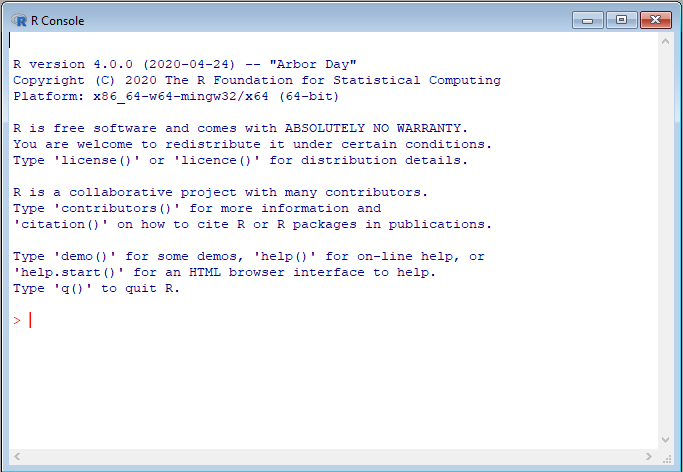
\includegraphics[keepaspectratio,alt={Screenshot of the R Terminal Window}]{images/rterminal.png}}

}

\caption{Screenshot of the R Terminal Window (Source:
{[}Wikipedia{]}(https://commons.wikimedia.org/w/index.php?curid=90393195))}

\end{figure}%

In practice, you will probably never use the R terminal to conduct your
research. Instead you will use \textbf{RStudio} which is an extremely
popular Integrated Development Environment (IDE). RStudio essentially
acts as an intermediate layer between the researcher and R that helps
make R much easier to use by providing a more structured and
user-friendly interface as well as a large number of additional
features, for example, \href{https://quarto.org}{Quarto} which allows us
to produce documents with code and output (such as this electronic
book). It looks like this:

\begin{figure}[H]

{\centering \pandocbounded{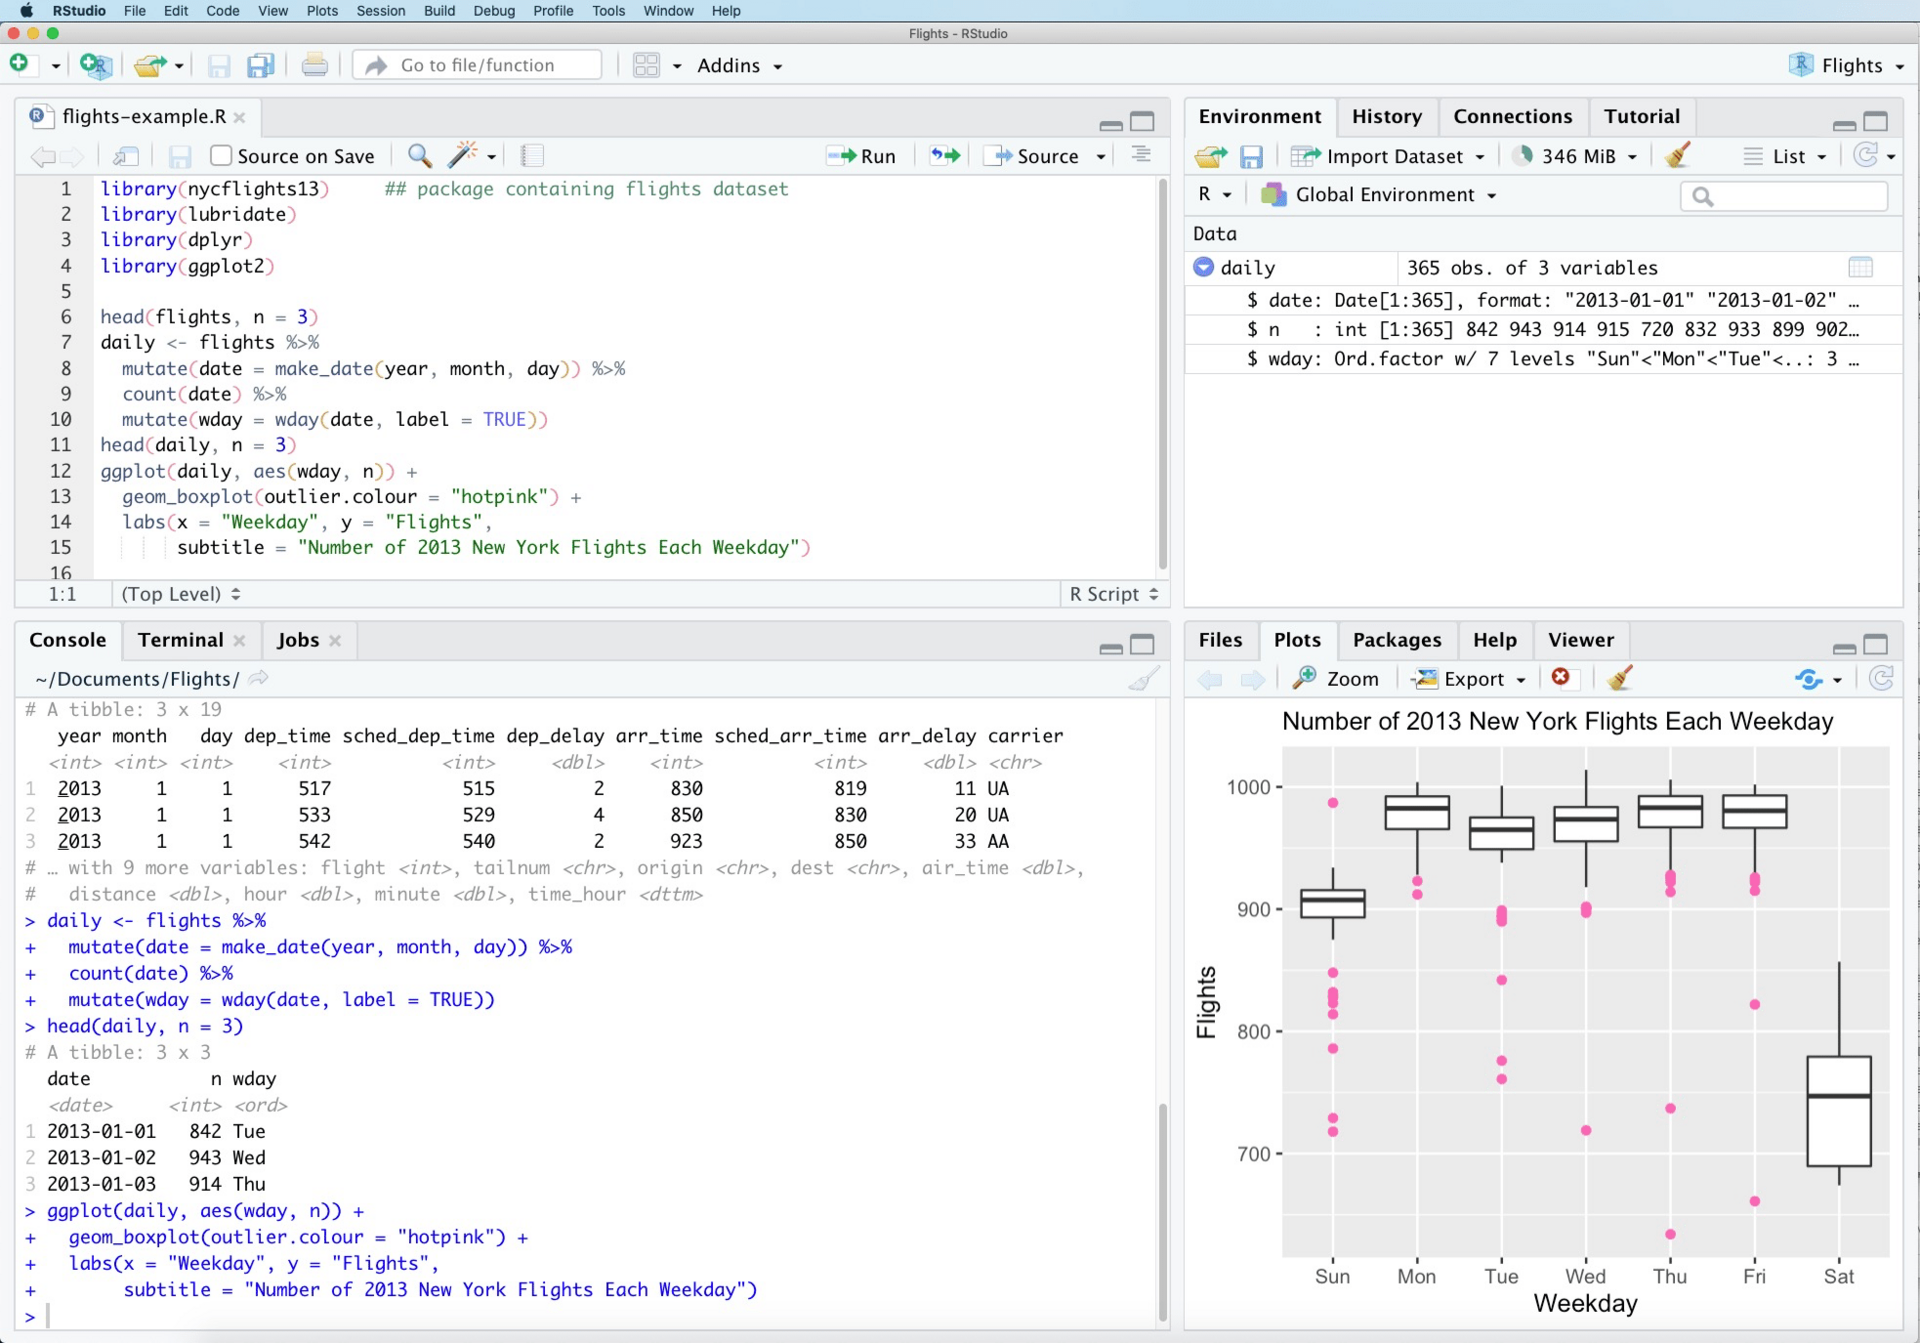
\includegraphics[keepaspectratio,alt={Screenshot of RStudio IDE window}]{images/rstudio.png}}

}

\caption{Screenshot of RStudio IDE window (Source:
\href{https://commons.wikimedia.org/w/index.php?curid=101293607}{Wikipedia})}

\end{figure}%

\subsubsection{Step 1: Install R}\label{step-1-install-r}

You can download R from \href{https://www.stats.bris.ac.uk/R/}{here} .
Choose the version that corresponds to your operative system
(Windows/Mac/Linux) and download the file.

Once downloaded, double-click the installation file and accept all the
default options.

\subsubsection{Step 2: Install R-Studio}\label{step-2-install-r-studio}

You can download RStudio from
\href{https://posit.co/download/rstudio-desktop/}{here}. Again, choose
the version that corresponds to your operative system, though the web
will probably recognise it automatically and give you the correct file.

If you prefer, here's a
\href{https://www.youtube.com/watch?v=ZvPFKfNHBNQ}{video guide} on how
to install R and RStudio and a
\href{https://www.youtube.com/watch?v=HWnanydsBCs.}{brief intro} to the
RStudio interface

\section{Other software you may want to
consider:}\label{other-software-you-may-want-to-consider}

Although, strictly speaking, only R and R-Studio are needed, there is
other software out there that you may find helpful in working towards
your assessment and even for your dissertation. This list may grow
throughout the semester.

\begin{itemize}
\item
  \href{https://www.zotero.org}{Zotero} - This is a powerful
  bibliography manager that helps you organise all of your references
  (articles, books, reports, websites, etc) as well as annotate them. It
  will also produce files that you can then use to produce formatted
  citations and lists of references when writing your work in either
  RStudio or Word.
\item
  \ldots{}
\end{itemize}

\section{Access to workshop data}\label{access-to-workshop-data}

In this module we will exclusively work with \textbf{secondary
datasets}. These are computer files that contain data previously
collected from human participants by researchers other than ourselves
and research agencies other than those we may work for or on behalf of
(in our case, the University). These datasets have in turn been made
publicly available in data repositories for other researchers to use for
purposes that may or may not be the same as those originally intended by
the data holders. Sometimes, such as for general surveys, questionnaires
are designed to include a long list of items such that the resulting
datasets enable researchers across different disciplines (sociology,
criminology, social policy, economics, political science, geography,
etc) to conduct analysis on very different topics.

In this module we will primarily work with datasets from the
\href{https://ukdataservice.ac.uk}{UK Data Service}, but to make things
easier the files will be made available to you via Minerva. Before
accessing the data files, you need \textbf{to sign the declaration in
the section {[}SPECIFY SECTION{]} on Minerva}.

To do this, follow this procedure

\subsection{Access to project (and dissertation?)
data}\label{access-to-project-and-dissertation-data}

Beyond the datasets we use in the workshops, you are likely to draw from
either the UK Data Service or other repositories (GESIS, ESS) to choose
a dataset for your assessment project.

There are however some access conditions and use restrictions that
researchers need to agree to comply with before they can get access to
such datasets. This is why you are expected to register your use of the
datasets and sign a declaration.

\url{https://ukdataservice.ac.uk/learning-hub/students/resources/data-for-your-project/}

and with the \href{https://www.europeansocialsurvey.org}{European Social
Survey}

t.

\url{https://ukdataservice.ac.uk/learning-hub/students/resources/data-for-your-project/}

\bookmarksetup{startatroot}

\chapter{Describing Continuous Data}\label{describing-continuous-data}

\bookmarksetup{startatroot}

\chapter{Describing Categorical data}\label{describing-categorical-data}

\section{Introduction}\label{introduction}

In this workshop we will get to grips with the basics of describing
categorical data using RStudio. To follow this guide you should have
first watched the video lectures on the VLE where each of the techniques
here used are discussed in detail. Also on the VLE, you will find
RStudio video tutorials that elaborate on this workshop guide.

The dataset we will analyse the ``2012 UK Omnibus Poverty and Social
Exclusion Survey: Necessities of Life'' which is an

\begin{quote}
`attitudinal survey aimed to identify what the population as a whole
think are 'necessities': things that everyone should be able to afford
and which no one should have to go without. Data were collected in
Northern Ireland Statistics and Research Agency (NISRA), and in Great
Britain (Scotland, England and Wales) by NatCen Social Research'.
\end{quote}

You can find the dataset and relevant documentation in the UK Data
Service by clicking this
\href{https://beta.ukdataservice.ac.uk/datacatalogue/studies/study?id=7878}{link}.
If interested in finding out more, you can read a report on the main
findings
\href{https://www.poverty.ac.uk/pse-research/what-do-we-think-we-need}{here}

The substantive questions that drive this workshop are:

\begin{enumerate}
\def\labelenumi{\arabic{enumi}.}
\tightlist
\item
  to what extent do UK residents regard a range of goods and services as
  necessary or merely desirable?
\item
  to what extent do perceptions of necessities vary across relevant
  socio-demographic groups?
\end{enumerate}

To answer these questions we will learn about and use in practice the
following analytical techniques:

\begin{itemize}
\tightlist
\item
  Numerical Summaries

  \begin{itemize}
  \tightlist
  \item
    Univariate frequency tables
  \item
    Bivariate contingency tables
  \end{itemize}
\item
  Visualisation

  \begin{itemize}
  \tightlist
  \item
    Univariate bar plots
  \item
    Bivariate clustered and Stacked bar plots
  \end{itemize}
\end{itemize}

You will notice that these are the very same techniques you learnt about
in the quantitative part of Level 2 Research Methods, so none of this
material should be new to you. Having said this, we will be able to
explore some aspects in a bit more detail to strengthen both your
intuitive and statistical understanding of what the techniques are
doing.

\section{Data and libraries}\label{data-and-libraries}

Assuming that you are already initialised RStudio in your computer and
you have opened a project located in a folder containing the dataset
file, the first steps is to load the dataset, call a number of packages
that are necessary to run the code for this workshop:

\begin{Shaded}
\begin{Highlighting}[]
\CommentTok{\# load R packages}
\FunctionTok{library}\NormalTok{(tidyverse)}
\FunctionTok{library}\NormalTok{(knitr)}
\FunctionTok{library}\NormalTok{(janitor)}
\FunctionTok{library}\NormalTok{(scales)}
\FunctionTok{library}\NormalTok{(ggstats)}

\CommentTok{\# load data}
\FunctionTok{load}\NormalTok{(}\StringTok{"pse\_omni.Rdata"}\NormalTok{)}
\end{Highlighting}
\end{Shaded}

If you want to have a quick look at the dataset to get a sense of what
it is like, you can use the functions \emph{glimpse() - list of
variables and values -} or \emph{view()} - the dataset in spreadsheet
form - with the dataset called \textbf{omni} - this is not shown in the
guide as it takes up multiple pages!

\begin{Shaded}
\begin{Highlighting}[]
\FunctionTok{glimpse}\NormalTok{(omni)}
\end{Highlighting}
\end{Shaded}

We will then move straight to the analysis.

\section{Numerical description of categorical
data:}\label{numerical-description-of-categorical-data}

\subsection{Base R}\label{base-r}

To describe the univariate distribution of a categorical variable we use
frequency tables. Frequency tables can be produced in R using the
function \textbf{table()} which can report both raw counts and
percentages depending on how we specify the code.

We begin by describing the univariate distribution as raw counts of
respondents for each category of the variable tv.

\begin{Shaded}
\begin{Highlighting}[]
\FunctionTok{table}\NormalTok{(omni}\SpecialCharTok{$}\NormalTok{tv)}
\end{Highlighting}
\end{Shaded}

\begin{verbatim}

Necessary Desirable 
     1013       892 
\end{verbatim}

The table shows that 1013 respondents say that having a TV is a
necessity whereas 892 answer that it is simply desirable.

Based on manipulating these raw counts we can calculate other
quantities. In order to manipulate this table we need to store it in
memory and give it a name, in this case \emph{tabtv}

\begin{Shaded}
\begin{Highlighting}[]
\CommentTok{\# We create an object call tabtv that contains the distribution of variable "tv" in the dataset omni}
\NormalTok{tabtv }\OtherTok{\textless{}{-}} \FunctionTok{table}\NormalTok{(omni}\SpecialCharTok{$}\NormalTok{tv)}

\CommentTok{\# We ask R to display the new object "tabtv"}
\NormalTok{tabtv}
\end{Highlighting}
\end{Shaded}

\begin{verbatim}

Necessary Desirable 
     1013       892 
\end{verbatim}

The first thing we can do is to add margins to the tabtv table -
i.e.~the sum of all observations contained in your table - using the
function \emph{addmargins()}

\begin{Shaded}
\begin{Highlighting}[]
\FunctionTok{addmargins}\NormalTok{(tabtv)}
\end{Highlighting}
\end{Shaded}

\begin{verbatim}

Necessary Desirable       Sum 
     1013       892      1905 
\end{verbatim}

We can also express the numbers in the table as proportions or
percentages

\begin{Shaded}
\begin{Highlighting}[]
\CommentTok{\# as proportion}
\FunctionTok{prop.table}\NormalTok{(tabtv)}
\end{Highlighting}
\end{Shaded}

\begin{verbatim}

Necessary Desirable 
0.5317585 0.4682415 
\end{verbatim}

\begin{Shaded}
\begin{Highlighting}[]
\CommentTok{\#as percentage}
\FunctionTok{prop.table}\NormalTok{(tabtv)}\SpecialCharTok{*}\DecValTok{100}
\end{Highlighting}
\end{Shaded}

\begin{verbatim}

Necessary Desirable 
 53.17585  46.82415 
\end{verbatim}

\subsection{Tidyverse}\label{tidyverse}

You can produce the same results using tidyverse functions. The
tidyverse is a family of packages that have consistent coding principles
and data handling conventions. For a detailed treatment of the tidyverse
see the book \href{https://r4ds.hadley.nz}{R for Data Science (2nd
Edition)} by Wickham, Çetinkaya-Rundel and Grolemund.

A key element of the tidyverse is the use of the pipe operator
\textbf{\textbar\textgreater{}} \emph{(hotkey: command/ctrl + shift +
m}) which allow us to write sequences or chains of functions - a bit
like a baking recipe as shown in figure 1.

\begin{figure}[H]

{\centering \includegraphics[width=3.67708in,height=\textheight,keepaspectratio]{images/Screenshot 2024-10-01 at 17.44.34.png}

}

\caption{Piping in R (@ArthurWelle)}

\end{figure}%

Here's an example of how we create a frequency table in R using
tidyverse functions or verbs and the pipe operator:

\begin{Shaded}
\begin{Highlighting}[]
\NormalTok{omni }\SpecialCharTok{|\textgreater{}} \CommentTok{\# dataset }
  \FunctionTok{drop\_na}\NormalTok{(tv) }\SpecialCharTok{|\textgreater{}} \CommentTok{\# drop missing values from variable tv}
  \FunctionTok{group\_by}\NormalTok{(tv) }\SpecialCharTok{|\textgreater{}} \CommentTok{\# across the response categories}
  \FunctionTok{summarise}\NormalTok{(}\AttributeTok{n =} \FunctionTok{n}\NormalTok{()) }\SpecialCharTok{|\textgreater{}} \CommentTok{\# count the respondents}
  \FunctionTok{mutate}\NormalTok{(}\AttributeTok{perc =}\NormalTok{ n }\SpecialCharTok{/} \FunctionTok{sum}\NormalTok{(n) }\SpecialCharTok{*} \DecValTok{100}\NormalTok{) }\SpecialCharTok{|\textgreater{}} 
  \FunctionTok{kable}\NormalTok{() }\CommentTok{\# render nice looking table}
\end{Highlighting}
\end{Shaded}

{\def\LTcaptype{none} % do not increment counter
\begin{longtable}[]{@{}lrr@{}}
\toprule\noalign{}
tv & n & perc \\
\midrule\noalign{}
\endhead
\bottomrule\noalign{}
\endlastfoot
Necessary & 1013 & 53.17585 \\
Desirable & 892 & 46.82415 \\
\end{longtable}
}

or using the function \emph{count()}

\begin{Shaded}
\begin{Highlighting}[]
\NormalTok{omni }\SpecialCharTok{|\textgreater{}} \CommentTok{\# dataset}
  \FunctionTok{drop\_na}\NormalTok{(tv) }\SpecialCharTok{|\textgreater{}} \CommentTok{\# drop missing values from variable tv}
  \FunctionTok{count}\NormalTok{(tv) }\SpecialCharTok{|\textgreater{}} \CommentTok{\# count the respondents in each category}
  \FunctionTok{mutate}\NormalTok{(}\AttributeTok{perc =}\NormalTok{ n }\SpecialCharTok{/} \FunctionTok{sum}\NormalTok{(n) }\SpecialCharTok{*} \DecValTok{100}\NormalTok{) }\SpecialCharTok{|\textgreater{}} 
  \FunctionTok{kable}\NormalTok{() }\CommentTok{\# render nice looking table}
\end{Highlighting}
\end{Shaded}

{\def\LTcaptype{none} % do not increment counter
\begin{longtable}[]{@{}lrr@{}}
\toprule\noalign{}
tv & n & perc \\
\midrule\noalign{}
\endhead
\bottomrule\noalign{}
\endlastfoot
Necessary & 1013 & 53.17585 \\
Desirable & 892 & 46.82415 \\
\end{longtable}
}

To round percentages up to 2 digits you can use the \emph{round()}
function

\begin{Shaded}
\begin{Highlighting}[]
\NormalTok{omni }\SpecialCharTok{|\textgreater{}} \CommentTok{\# dataset}
  \FunctionTok{drop\_na}\NormalTok{(tv) }\SpecialCharTok{|\textgreater{}} \CommentTok{\# drop missing values from variable tv}
  \FunctionTok{count}\NormalTok{(tv) }\SpecialCharTok{|\textgreater{}} \CommentTok{\# count the respondents in each category}
  \FunctionTok{mutate}\NormalTok{(}\AttributeTok{perc =} \FunctionTok{round}\NormalTok{(n }\SpecialCharTok{/} \FunctionTok{sum}\NormalTok{(n) }\SpecialCharTok{*} \DecValTok{100}\NormalTok{, }\DecValTok{2}\NormalTok{)) }\SpecialCharTok{|\textgreater{}} \CommentTok{\# calculate percentage}
  \FunctionTok{kable}\NormalTok{() }\CommentTok{\# render nice looking table}
\end{Highlighting}
\end{Shaded}

{\def\LTcaptype{none} % do not increment counter
\begin{longtable}[]{@{}lrr@{}}
\toprule\noalign{}
tv & n & perc \\
\midrule\noalign{}
\endhead
\bottomrule\noalign{}
\endlastfoot
Necessary & 1013 & 53.18 \\
Desirable & 892 & 46.82 \\
\end{longtable}
}

Or you can use the function \emph{percent} from the package
\textbf{scales} which will also add the \% sign

\begin{Shaded}
\begin{Highlighting}[]
\NormalTok{omni }\SpecialCharTok{|\textgreater{}} \CommentTok{\# dataset}
  \FunctionTok{drop\_na}\NormalTok{(tv) }\SpecialCharTok{|\textgreater{}} \CommentTok{\# drop missing values from variable tv}
  \FunctionTok{count}\NormalTok{(tv) }\SpecialCharTok{|\textgreater{}} \CommentTok{\# count the respondents in each category}
  \FunctionTok{mutate}\NormalTok{(}\AttributeTok{perc =} \FunctionTok{percent}\NormalTok{(n }\SpecialCharTok{/} \FunctionTok{sum}\NormalTok{(n), }\FloatTok{0.01}\NormalTok{)) }\SpecialCharTok{|\textgreater{}} \CommentTok{\# calculate percentage}
  \FunctionTok{kable}\NormalTok{() }\CommentTok{\# render nice looking table}
\end{Highlighting}
\end{Shaded}

{\def\LTcaptype{none} % do not increment counter
\begin{longtable}[]{@{}lrl@{}}
\toprule\noalign{}
tv & n & perc \\
\midrule\noalign{}
\endhead
\bottomrule\noalign{}
\endlastfoot
Necessary & 1013 & 53.18\% \\
Desirable & 892 & 46.82\% \\
\end{longtable}
}

Finally, the \emph{tabyl} function (from the \textbf{janitor} package)
makes it quite easy to produce nice tables, which becomes particularly
useful for contingency tables discussed further below.

\begin{Shaded}
\begin{Highlighting}[]
\NormalTok{omni }\SpecialCharTok{|\textgreater{}} 
  \FunctionTok{drop\_na}\NormalTok{(tv) }\SpecialCharTok{|\textgreater{}} 
  \FunctionTok{tabyl}\NormalTok{(tv) }\SpecialCharTok{|\textgreater{}} \CommentTok{\# create frequency table}
  \FunctionTok{adorn\_pct\_formatting}\NormalTok{(}\AttributeTok{digits =} \DecValTok{1}\NormalTok{) }\SpecialCharTok{|\textgreater{}} \CommentTok{\# choose number of decimals}
  \FunctionTok{kable}\NormalTok{()}
\end{Highlighting}
\end{Shaded}

{\def\LTcaptype{none} % do not increment counter
\begin{longtable}[]{@{}lrl@{}}
\toprule\noalign{}
tv & n & percent \\
\midrule\noalign{}
\endhead
\bottomrule\noalign{}
\endlastfoot
Necessary & 1013 & 53.2\% \\
Desirable & 892 & 46.8\% \\
\end{longtable}
}

\section{Graphical representation of univariate categorical
data:}\label{graphical-representation-of-univariate-categorical-data}

With ggplot we can create bar charts easily using the \emph{geom\_bar}
option. The basic syntax is as follows:

\begin{Shaded}
\begin{Highlighting}[]
\CommentTok{\# Basic barplot}
\FunctionTok{ggplot}\NormalTok{(}\AttributeTok{data =}\NormalTok{ omni, }\FunctionTok{aes}\NormalTok{(}\AttributeTok{x =}\NormalTok{ tv)) }\SpecialCharTok{+}
  \FunctionTok{geom\_bar}\NormalTok{(}\AttributeTok{stat =} \StringTok{"count"}\NormalTok{)}
\end{Highlighting}
\end{Shaded}

\pandocbounded{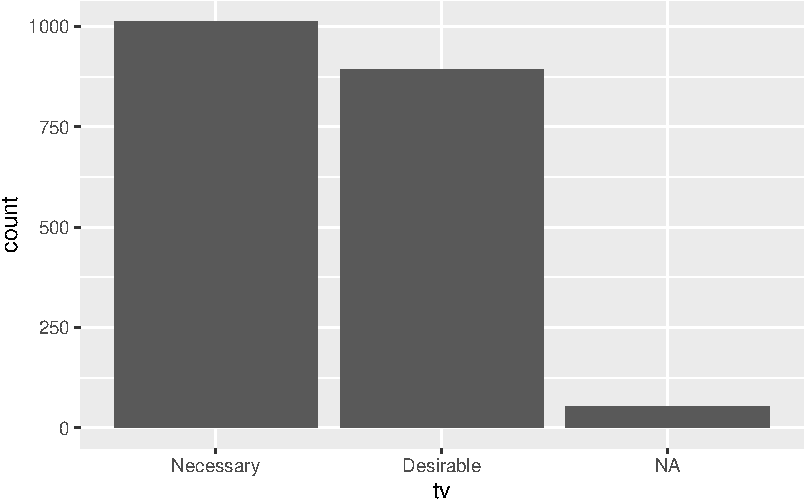
\includegraphics[keepaspectratio]{03_categorical_files/figure-pdf/unnamed-chunk-12-1.pdf}}

Notice that R ggplot creates a bar for the missing values (called NA).
This NA bar draws away our attention from the Necessary and Desirable
bars and could potentially distort the plot as a whole. We will remove
the missing values by subsetting the data we input into the graph. To
subset the data we use the following line when defining the data in
ggplot: \textbf{omni{[}!is.na(omni\$tv), {]}}

\begin{Shaded}
\begin{Highlighting}[]
\CommentTok{\# Eliminate missing value category from the chart with (omni[!is.na(omni$tv), ]}
\FunctionTok{ggplot}\NormalTok{(omni[}\SpecialCharTok{!}\FunctionTok{is.na}\NormalTok{(omni}\SpecialCharTok{$}\NormalTok{tv), ], }\FunctionTok{aes}\NormalTok{(}\AttributeTok{x=}\NormalTok{tv)) }\SpecialCharTok{+}
  \FunctionTok{geom\_bar}\NormalTok{(}\AttributeTok{stat=}\StringTok{"count"}\NormalTok{)}
\end{Highlighting}
\end{Shaded}

\pandocbounded{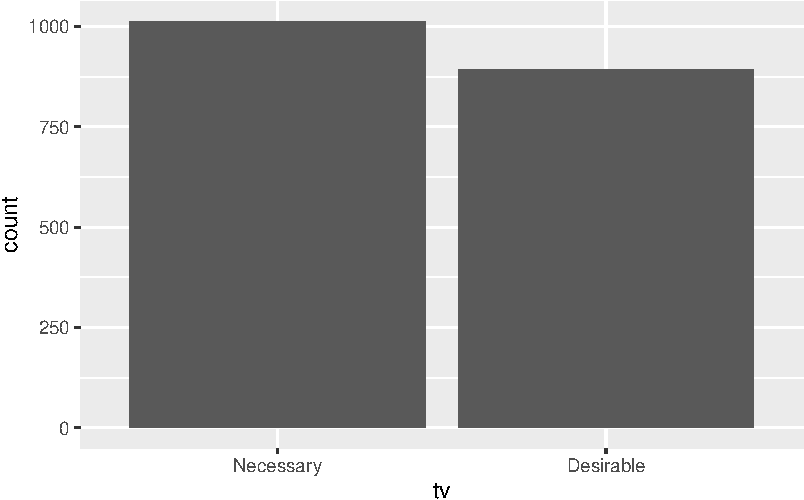
\includegraphics[keepaspectratio]{03_categorical_files/figure-pdf/unnamed-chunk-13-1.pdf}}

Alternatively we can use the function \textbf{complete.cases()} which is
a bit more readable and produces the same result:

\begin{Shaded}
\begin{Highlighting}[]
\CommentTok{\# Eliminate missing value category from the chart with (omni[complete.cases(omni$tv), ]}
\FunctionTok{ggplot}\NormalTok{(omni[}\FunctionTok{complete.cases}\NormalTok{(omni}\SpecialCharTok{$}\NormalTok{tv), ], }\FunctionTok{aes}\NormalTok{(}\AttributeTok{x=}\NormalTok{tv)) }\SpecialCharTok{+}
  \FunctionTok{geom\_bar}\NormalTok{(}\AttributeTok{stat=}\StringTok{"count"}\NormalTok{)}
\end{Highlighting}
\end{Shaded}

\pandocbounded{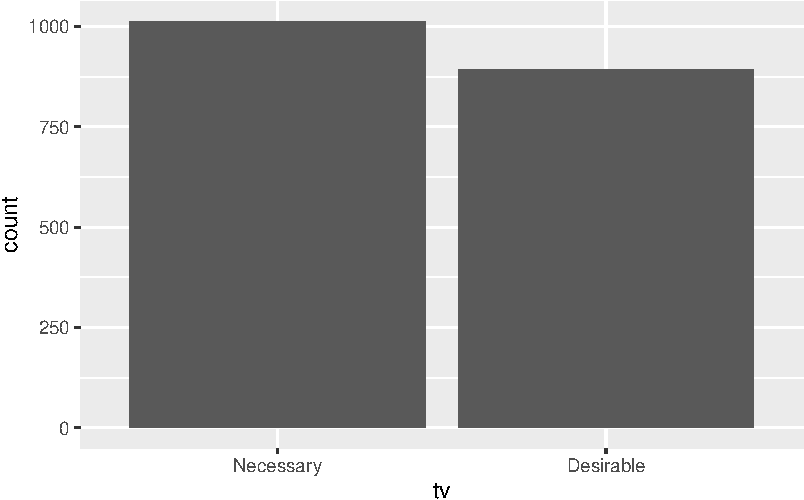
\includegraphics[keepaspectratio]{03_categorical_files/figure-pdf/unnamed-chunk-14-1.pdf}}

Often you may want to plot proportions rather than counts, which can be
achieved by changing the aesthetics' options. In this case, after
declaring the variables write a \textbf{comma} and add
\textbf{after\_stat(prop), group = 1}:

\begin{Shaded}
\begin{Highlighting}[]
\FunctionTok{ggplot}\NormalTok{(}\AttributeTok{data =}\NormalTok{ omni[}\FunctionTok{complete.cases}\NormalTok{(omni}\SpecialCharTok{$}\NormalTok{tv), ], }\FunctionTok{aes}\NormalTok{(}\AttributeTok{x=}\NormalTok{tv, }\AttributeTok{y =} \FunctionTok{after\_stat}\NormalTok{(prop), }\AttributeTok{group =} \DecValTok{1}\NormalTok{)) }\SpecialCharTok{+}
  \FunctionTok{geom\_bar}\NormalTok{(}\AttributeTok{stat=}\StringTok{"count"}\NormalTok{) }
\end{Highlighting}
\end{Shaded}

\pandocbounded{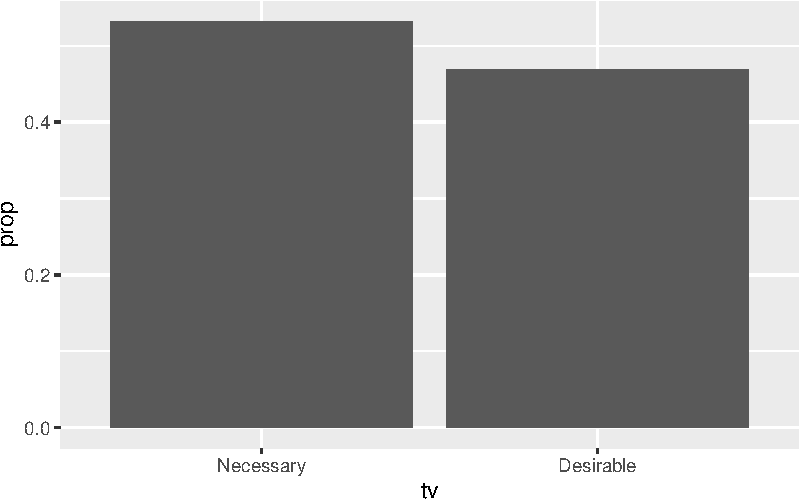
\includegraphics[keepaspectratio]{03_categorical_files/figure-pdf/unnamed-chunk-15-1.pdf}}

Since percentages are basically proportions multiplied by 100, we can
have percentages on our plot by re-scaling (changing the scale) of the
vertical axis using the option \emph{scale\_y\_continuous(labels =
scales::percent)}

\begin{Shaded}
\begin{Highlighting}[]
\CommentTok{\# If you want proportions, you need to modify the aesthetics options for the y axis}

\FunctionTok{ggplot}\NormalTok{(}\AttributeTok{data =}\NormalTok{ omni[}\FunctionTok{complete.cases}\NormalTok{(omni}\SpecialCharTok{$}\NormalTok{tv), ], }
       \FunctionTok{aes}\NormalTok{(}\AttributeTok{x=}\NormalTok{tv, }\AttributeTok{y =} \FunctionTok{after\_stat}\NormalTok{(prop), }\AttributeTok{group =} \DecValTok{1}\NormalTok{)) }\SpecialCharTok{+}
  \FunctionTok{geom\_bar}\NormalTok{(}\AttributeTok{stat=}\StringTok{"count"}\NormalTok{) }\SpecialCharTok{+} 
  \FunctionTok{scale\_y\_continuous}\NormalTok{(}\AttributeTok{labels =}\NormalTok{ scales}\SpecialCharTok{::}\NormalTok{percent)}
\end{Highlighting}
\end{Shaded}

\pandocbounded{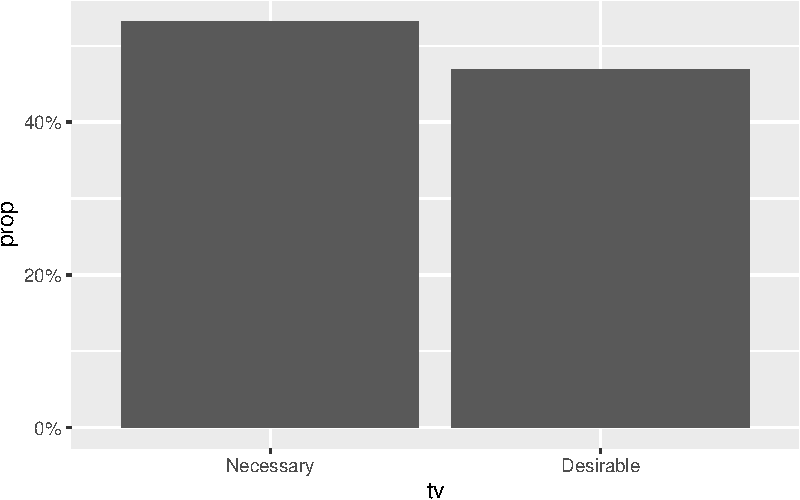
\includegraphics[keepaspectratio]{03_categorical_files/figure-pdf/unnamed-chunk-16-1.pdf}}

Or using the \textbf{tidyverse} you can integrate the specification of
the ggplot graphs as part of a wider sequence of functions applied to
the same data:

\begin{Shaded}
\begin{Highlighting}[]
\NormalTok{omni }\SpecialCharTok{|\textgreater{}} 
  \FunctionTok{drop\_na}\NormalTok{(tv) }\SpecialCharTok{|\textgreater{}} 
  \FunctionTok{ggplot}\NormalTok{() }\SpecialCharTok{+}
  \FunctionTok{geom\_bar}\NormalTok{(}\FunctionTok{aes}\NormalTok{( }\AttributeTok{x =}\NormalTok{ tv, }\AttributeTok{y =} \FunctionTok{after\_stat}\NormalTok{(prop), }\AttributeTok{group =} \DecValTok{1}\NormalTok{)) }\SpecialCharTok{+}
  \FunctionTok{scale\_y\_continuous}\NormalTok{(}\AttributeTok{labels =}\NormalTok{ scales}\SpecialCharTok{::}\NormalTok{percent)}
\end{Highlighting}
\end{Shaded}

\pandocbounded{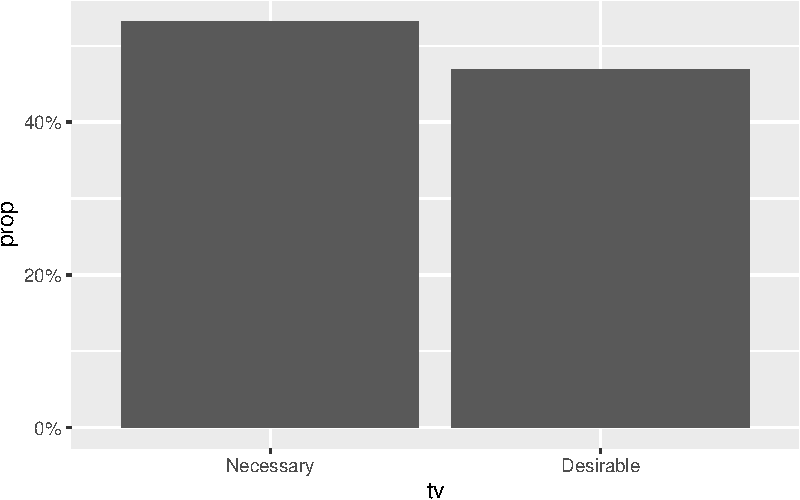
\includegraphics[keepaspectratio]{03_categorical_files/figure-pdf/unnamed-chunk-17-1.pdf}}

Finally, we should change the labels in the plot and add a title to make
it more informative

\begin{Shaded}
\begin{Highlighting}[]
\NormalTok{omni }\SpecialCharTok{|\textgreater{}} 
  \FunctionTok{drop\_na}\NormalTok{(tv) }\SpecialCharTok{|\textgreater{}} 
  \FunctionTok{ggplot}\NormalTok{() }\SpecialCharTok{+}
  \FunctionTok{geom\_bar}\NormalTok{(}\FunctionTok{aes}\NormalTok{( }\AttributeTok{x =}\NormalTok{ tv, }\AttributeTok{y =} \FunctionTok{after\_stat}\NormalTok{(prop), }\AttributeTok{group =} \DecValTok{1}\NormalTok{)) }\SpecialCharTok{+}
  \FunctionTok{scale\_y\_continuous}\NormalTok{(}\AttributeTok{labels =}\NormalTok{ scales}\SpecialCharTok{::}\NormalTok{percent) }\SpecialCharTok{+}
  \FunctionTok{xlab}\NormalTok{(}\StringTok{"Is a TV set necessary?"}\NormalTok{) }\SpecialCharTok{+} \CommentTok{\# change the x axis label}
  \FunctionTok{ylab}\NormalTok{(}\StringTok{"Percentage of respondents"}\NormalTok{) }\SpecialCharTok{+} \CommentTok{\# change the y axis label}
  \FunctionTok{ggtitle}\NormalTok{(}\StringTok{"A majority of respondents think a TV is necessary"}\NormalTok{) }\CommentTok{\# change the main title of the graph}
\end{Highlighting}
\end{Shaded}

\pandocbounded{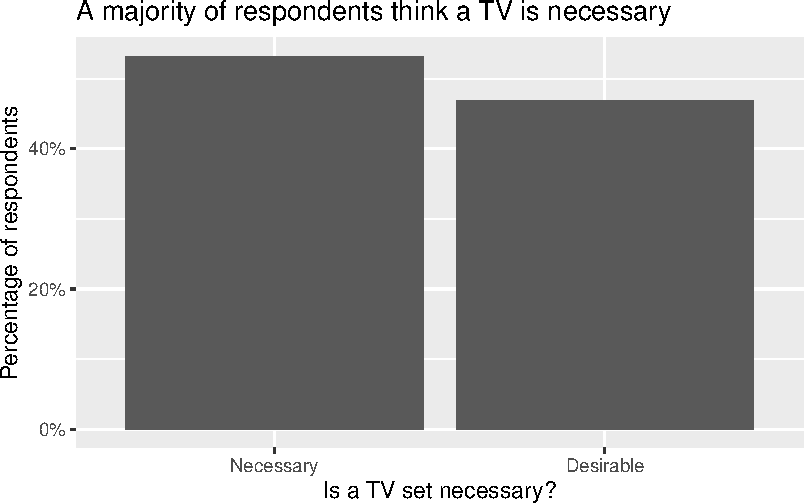
\includegraphics[keepaspectratio]{03_categorical_files/figure-pdf/unnamed-chunk-18-1.pdf}}

You can also use specify labels and title within the function
\textbf{labs} and produce the exact same results:

\begin{Shaded}
\begin{Highlighting}[]
\NormalTok{omni }\SpecialCharTok{|\textgreater{}} 
  \FunctionTok{drop\_na}\NormalTok{(tv) }\SpecialCharTok{|\textgreater{}} 
  \FunctionTok{ggplot}\NormalTok{() }\SpecialCharTok{+}
  \FunctionTok{geom\_bar}\NormalTok{(}\FunctionTok{aes}\NormalTok{( }\AttributeTok{x =}\NormalTok{ tv, }\AttributeTok{y =} \FunctionTok{after\_stat}\NormalTok{(prop), }\AttributeTok{group =} \DecValTok{1}\NormalTok{)) }\SpecialCharTok{+}
  \FunctionTok{labs}\NormalTok{(}\AttributeTok{x =} \StringTok{"Is a TV set necessary?"}\NormalTok{, }\CommentTok{\# specify x{-}axis lab}
       \AttributeTok{y =} \StringTok{"Percentage of respondents"}\NormalTok{, }\CommentTok{\# specify y{-}axis lab}
       \AttributeTok{caption =} \StringTok{"Poverty and Social Exclusion Survey 2012"}\NormalTok{,}
       \AttributeTok{title =} \StringTok{"A majority of respondents think a TV is necessary"}\NormalTok{)  }\CommentTok{\# main title}
\end{Highlighting}
\end{Shaded}

\pandocbounded{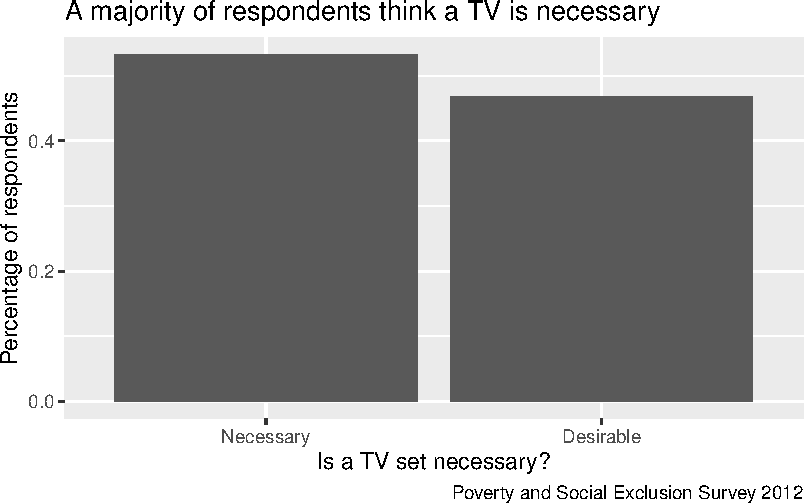
\includegraphics[keepaspectratio]{03_categorical_files/figure-pdf/unnamed-chunk-19-1.pdf}}

\section{Exercise I}\label{exercise-i}

Provide the code necessary to calculate and plot the univariate
distribution (as counts and percentages) of respondents according to
whether they think having a ``a damp-free house'' (variable
\emph{nodamp}) is necessary as opposed to just desirable. You should
obtain the following results:

\begin{verbatim}

Necessary Desirable 
    94.47      5.53 
\end{verbatim}

{\def\LTcaptype{none} % do not increment counter
\begin{longtable}[]{@{}lrr@{}}
\toprule\noalign{}
nodamp & n & percent \\
\midrule\noalign{}
\endhead
\bottomrule\noalign{}
\endlastfoot
Necessary & 1811 & 94.470527 \\
Desirable & 106 & 5.529473 \\
\end{longtable}
}

\pandocbounded{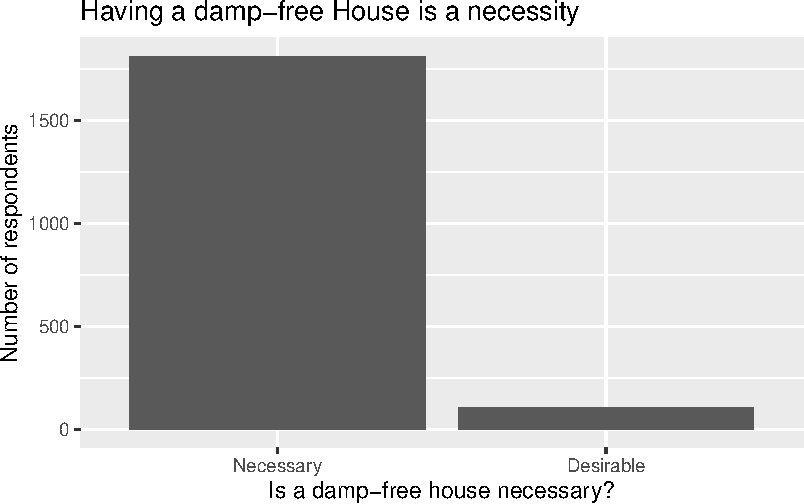
\includegraphics[keepaspectratio]{03_categorical_files/figure-pdf/unnamed-chunk-20-1.pdf}}

\pandocbounded{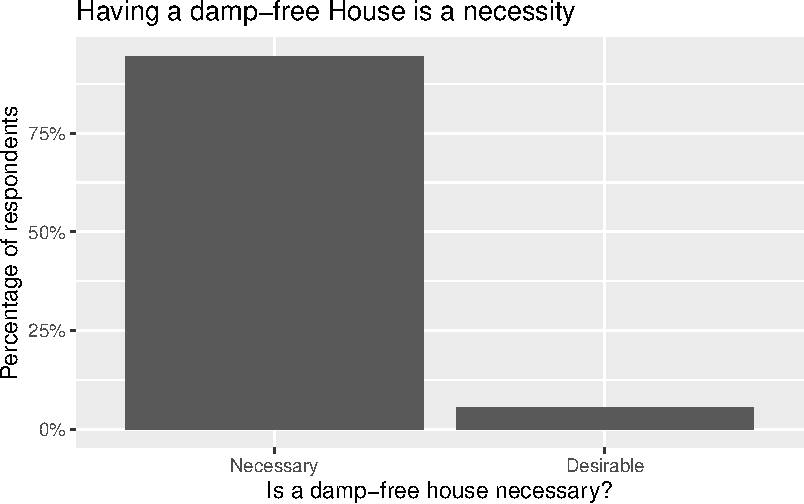
\includegraphics[keepaspectratio]{03_categorical_files/figure-pdf/unnamed-chunk-20-2.pdf}}

\section{Working with bivariate categorical
data}\label{working-with-bivariate-categorical-data}

After learning how to produce a frequency table, we move onto
contingency tables or crosstabulations. Contingency tables help us
represent the cross-classification of two or more categorical variables
- i.e.~how individuals are classified simultaneously in the categories
of more than one variable.

For instance, we may want to find out whether one's perception of TV as
a necessity or a mere desire depends on past employment status. Not
unlike the comparisons of pay between men and women (or levels of
educational achievement) here we also compare the distribution of
attitudes towards different goods between individuals classified in
different socioeconomic categories.

\subsection{Base R}\label{base-r-1}

We use again the function \textbf{table()} but this time we specify 2
variables as \textbf{table(var1, var2)}.

\begin{Shaded}
\begin{Highlighting}[]
\FunctionTok{table}\NormalTok{(omni}\SpecialCharTok{$}\NormalTok{paidwork, omni}\SpecialCharTok{$}\NormalTok{tv)}
\end{Highlighting}
\end{Shaded}

\begin{verbatim}
     
      Necessary Desirable
  Yes       438       516
  No        571       365
\end{verbatim}

Notice how now we obtain the marginal values for each category.

\begin{Shaded}
\begin{Highlighting}[]
\NormalTok{tvpw}\OtherTok{\textless{}{-}}\FunctionTok{table}\NormalTok{(omni}\SpecialCharTok{$}\NormalTok{paidwork, omni}\SpecialCharTok{$}\NormalTok{tv) }\CommentTok{\# create table object}
\FunctionTok{addmargins}\NormalTok{(tvpw) }\CommentTok{\# add row, column and total sums}
\end{Highlighting}
\end{Shaded}

\begin{verbatim}
     
      Necessary Desirable  Sum
  Yes       438       516  954
  No        571       365  936
  Sum      1009       881 1890
\end{verbatim}

It may be difficult to make sense of the raw counts, so it is often
desirable to include either row or column proportions or percentages.
This is easily done

\begin{Shaded}
\begin{Highlighting}[]
\CommentTok{\# row percentages}
\FunctionTok{prop.table}\NormalTok{(tvpw, }\DecValTok{1}\NormalTok{)}\SpecialCharTok{*}\DecValTok{100}
\end{Highlighting}
\end{Shaded}

\begin{verbatim}
     
      Necessary Desirable
  Yes  45.91195  54.08805
  No   61.00427  38.99573
\end{verbatim}

\begin{Shaded}
\begin{Highlighting}[]
\CommentTok{\#column percentages (re{-}arrange the table with omni$tv in the rows)}
\NormalTok{tvpw\_inv}\OtherTok{\textless{}{-}}\FunctionTok{table}\NormalTok{(omni}\SpecialCharTok{$}\NormalTok{tv, omni}\SpecialCharTok{$}\NormalTok{paidwork)}
\FunctionTok{prop.table}\NormalTok{(tvpw\_inv, }\DecValTok{2}\NormalTok{)}\SpecialCharTok{*}\DecValTok{100}
\end{Highlighting}
\end{Shaded}

\begin{verbatim}
           
                 Yes       No
  Necessary 45.91195 61.00427
  Desirable 54.08805 38.99573
\end{verbatim}

\subsection{Tidyverse}\label{tidyverse-1}

We can achieve the same using tidyverse code, though it is decidedly
more involved:

\begin{Shaded}
\begin{Highlighting}[]
\NormalTok{omni }\SpecialCharTok{|\textgreater{}} 
  \FunctionTok{drop\_na}\NormalTok{(paidwork, tv) }\SpecialCharTok{|\textgreater{}} \CommentTok{\# remove missing values on two vars}
  \FunctionTok{group\_by}\NormalTok{(paidwork, tv) }\SpecialCharTok{|\textgreater{}} \CommentTok{\#arrange by the categories of two vars}
  \FunctionTok{summarise}\NormalTok{(}\AttributeTok{n =} \FunctionTok{n}\NormalTok{()) }\SpecialCharTok{|\textgreater{}}  \CommentTok{\# count respondents in each combination}
  \FunctionTok{spread}\NormalTok{(tv, n) }\SpecialCharTok{|\textgreater{}} \CommentTok{\# organise them as contingency table}
  \FunctionTok{adorn\_totals}\NormalTok{(}\FunctionTok{c}\NormalTok{(}\StringTok{"row"}\NormalTok{, }\StringTok{"col"}\NormalTok{)) }\SpecialCharTok{|\textgreater{}} \CommentTok{\#add margins from tabyl}
  \FunctionTok{kable}\NormalTok{()}
\end{Highlighting}
\end{Shaded}

{\def\LTcaptype{none} % do not increment counter
\begin{longtable}[]{@{}lrrr@{}}
\toprule\noalign{}
paidwork & Necessary & Desirable & Total \\
\midrule\noalign{}
\endhead
\bottomrule\noalign{}
\endlastfoot
Yes & 438 & 516 & 954 \\
No & 571 & 365 & 936 \\
Total & 1009 & 881 & 1890 \\
\end{longtable}
}

For row percentages you would use:

\begin{Shaded}
\begin{Highlighting}[]
\NormalTok{omni }\SpecialCharTok{|\textgreater{}} 
  \FunctionTok{drop\_na}\NormalTok{(paidwork, tv) }\SpecialCharTok{|\textgreater{}} 
  \FunctionTok{group\_by}\NormalTok{(paidwork, tv) }\SpecialCharTok{|\textgreater{}}
  \FunctionTok{summarise}\NormalTok{(}\AttributeTok{n =} \FunctionTok{n}\NormalTok{()) }\SpecialCharTok{|\textgreater{}} 
  \FunctionTok{mutate}\NormalTok{(}\AttributeTok{prop=}\NormalTok{n}\SpecialCharTok{/}\FunctionTok{sum}\NormalTok{(n)) }\SpecialCharTok{|\textgreater{}} 
  \FunctionTok{select}\NormalTok{(}\SpecialCharTok{{-}}\NormalTok{n) }\SpecialCharTok{|\textgreater{}} 
  \FunctionTok{spread}\NormalTok{(tv, prop) }\SpecialCharTok{|\textgreater{}} 
  \FunctionTok{kable}\NormalTok{()}
\end{Highlighting}
\end{Shaded}

{\def\LTcaptype{none} % do not increment counter
\begin{longtable}[]{@{}lrr@{}}
\toprule\noalign{}
paidwork & Necessary & Desirable \\
\midrule\noalign{}
\endhead
\bottomrule\noalign{}
\endlastfoot
Yes & 0.4591195 & 0.5408805 \\
No & 0.6100427 & 0.3899573 \\
\end{longtable}
}

For column percentages you could use:

\begin{Shaded}
\begin{Highlighting}[]
\NormalTok{omni }\SpecialCharTok{|\textgreater{}} 
  \FunctionTok{drop\_na}\NormalTok{(paidwork, tv) }\SpecialCharTok{|\textgreater{}} 
  \FunctionTok{group\_by}\NormalTok{(tv, paidwork) }\SpecialCharTok{|\textgreater{}} 
  \FunctionTok{summarise}\NormalTok{(}\AttributeTok{n =} \FunctionTok{n}\NormalTok{()) }\SpecialCharTok{|\textgreater{}} 
  \FunctionTok{mutate}\NormalTok{(}\AttributeTok{prop=}\NormalTok{n}\SpecialCharTok{/}\FunctionTok{sum}\NormalTok{(n)) }\SpecialCharTok{|\textgreater{}} 
  \FunctionTok{select}\NormalTok{(}\SpecialCharTok{{-}}\NormalTok{n) }\SpecialCharTok{|\textgreater{}} 
  \FunctionTok{spread}\NormalTok{(tv, prop) }\SpecialCharTok{|\textgreater{}} 
  \FunctionTok{kable}\NormalTok{()}
\end{Highlighting}
\end{Shaded}

{\def\LTcaptype{none} % do not increment counter
\begin{longtable}[]{@{}lrr@{}}
\toprule\noalign{}
paidwork & Necessary & Desirable \\
\midrule\noalign{}
\endhead
\bottomrule\noalign{}
\endlastfoot
Yes & 0.4340932 & 0.5856981 \\
No & 0.5659068 & 0.4143019 \\
\end{longtable}
}

Finally, you could use \emph{tabyl()} for row percentages

\begin{Shaded}
\begin{Highlighting}[]
\NormalTok{omni }\SpecialCharTok{|\textgreater{}} 
  \FunctionTok{drop\_na}\NormalTok{(paidwork, tv) }\SpecialCharTok{|\textgreater{}} 
  \FunctionTok{tabyl}\NormalTok{(paidwork, tv) }\SpecialCharTok{|\textgreater{}} 
  \FunctionTok{adorn\_totals}\NormalTok{(}\FunctionTok{c}\NormalTok{(}\StringTok{"row"}\NormalTok{, }\StringTok{"col"}\NormalTok{)) }\SpecialCharTok{|\textgreater{}} 
  \FunctionTok{adorn\_percentages}\NormalTok{(}\StringTok{"row"}\NormalTok{) }\SpecialCharTok{|\textgreater{}} 
  \FunctionTok{adorn\_pct\_formatting}\NormalTok{(}\AttributeTok{digits =} \DecValTok{1}\NormalTok{) }\SpecialCharTok{|\textgreater{}} 
  \FunctionTok{adorn\_ns}\NormalTok{() }\SpecialCharTok{|\textgreater{}} 
  \FunctionTok{adorn\_title}\NormalTok{() }\SpecialCharTok{|\textgreater{}} 
  \FunctionTok{kable}\NormalTok{()}
\end{Highlighting}
\end{Shaded}

{\def\LTcaptype{none} % do not increment counter
\begin{longtable}[]{@{}llll@{}}
\toprule\noalign{}
& tv & & \\
\midrule\noalign{}
\endhead
\bottomrule\noalign{}
\endlastfoot
paidwork & Necessary & Desirable & Total \\
Yes & 45.9\% (438) & 54.1\% (516) & 100.0\% (954) \\
No & 61.0\% (571) & 39.0\% (365) & 100.0\% (936) \\
Total & 53.4\% (1,009) & 46.6\% (881) & 100.0\% (1,890) \\
\end{longtable}
}

Or column percentages

\begin{Shaded}
\begin{Highlighting}[]
\NormalTok{omni }\SpecialCharTok{|\textgreater{}} 
  \FunctionTok{drop\_na}\NormalTok{(paidwork, tv) }\SpecialCharTok{|\textgreater{}} 
  \FunctionTok{tabyl}\NormalTok{(paidwork, tv) }\SpecialCharTok{|\textgreater{}} 
  \FunctionTok{adorn\_totals}\NormalTok{(}\FunctionTok{c}\NormalTok{(}\StringTok{"row"}\NormalTok{, }\StringTok{"col"}\NormalTok{)) }\SpecialCharTok{|\textgreater{}} 
  \FunctionTok{adorn\_percentages}\NormalTok{(}\StringTok{"col"}\NormalTok{) }\SpecialCharTok{|\textgreater{}} 
  \FunctionTok{adorn\_pct\_formatting}\NormalTok{(}\AttributeTok{digits =} \DecValTok{1}\NormalTok{) }\SpecialCharTok{|\textgreater{}} 
  \FunctionTok{adorn\_ns}\NormalTok{() }\SpecialCharTok{|\textgreater{}} 
  \FunctionTok{adorn\_title}\NormalTok{() }\SpecialCharTok{|\textgreater{}} 
  \FunctionTok{kable}\NormalTok{()}
\end{Highlighting}
\end{Shaded}

{\def\LTcaptype{none} % do not increment counter
\begin{longtable}[]{@{}llll@{}}
\toprule\noalign{}
& tv & & \\
\midrule\noalign{}
\endhead
\bottomrule\noalign{}
\endlastfoot
paidwork & Necessary & Desirable & Total \\
Yes & 43.4\% (438) & 58.6\% (516) & 50.5\% (954) \\
No & 56.6\% (571) & 41.4\% (365) & 49.5\% (936) \\
Total & 100.0\% (1,009) & 100.0\% (881) & 100.0\% (1,890) \\
\end{longtable}
}

\section{Graphical representation of bivariate categorical
data:}\label{graphical-representation-of-bivariate-categorical-data}

Contingency tables can also be represented graphically using bar plots,
but the bars have to be plotted for each of the categories of the
independent variable separately. This means we need to think carefully
about what is the substantive nature of the relationship between both
variables. Thus we may want to know:

\begin{enumerate}
\def\labelenumi{\arabic{enumi}.}
\tightlist
\item
  How the distribution of perception of necessities varies between
  different economic positions.
\item
  The socioeconomic composition of those who think TVs are necessary
  compared to those that think TVs are only desirable goods.
\end{enumerate}

The first seems to be a more plausible relation. It makes sense that we
should care whether people with greater attachment to the labour market
are more or less likely to consider TVs a necessity compared to those
without.

The first bar plot we will create is a stacked bar chart.

\begin{Shaded}
\begin{Highlighting}[]
\CommentTok{\#stacked bar chart}
\FunctionTok{ggplot}\NormalTok{(}\AttributeTok{data =}\NormalTok{ omni[}\FunctionTok{complete.cases}\NormalTok{(omni}\SpecialCharTok{$}\NormalTok{tv) }\SpecialCharTok{\&} \SpecialCharTok{!}\FunctionTok{is.na}\NormalTok{(omni}\SpecialCharTok{$}\NormalTok{paidwork) ,] , }
       \FunctionTok{aes}\NormalTok{(}\AttributeTok{x=}\NormalTok{paidwork)) }\SpecialCharTok{+}
  \FunctionTok{geom\_bar}\NormalTok{(}\AttributeTok{stat=}\StringTok{"count"}\NormalTok{, }\FunctionTok{aes}\NormalTok{(}\AttributeTok{fill=}\NormalTok{tv)) }
\end{Highlighting}
\end{Shaded}

\pandocbounded{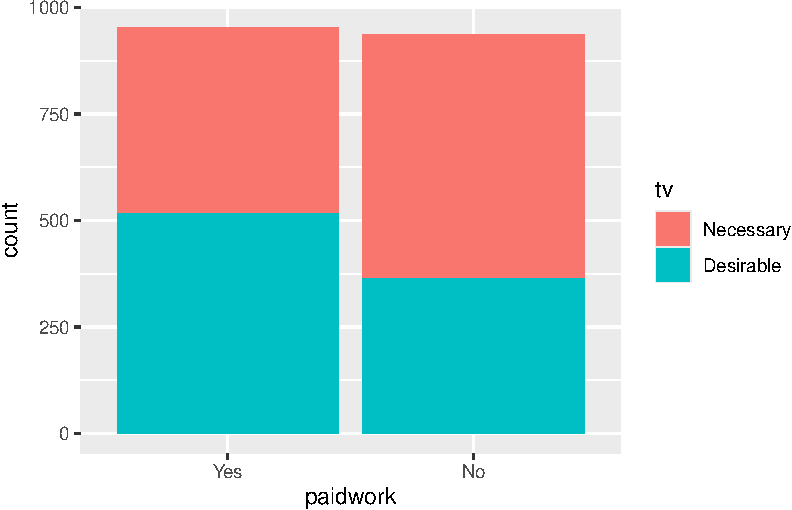
\includegraphics[keepaspectratio]{03_categorical_files/figure-pdf/unnamed-chunk-29-1.pdf}}

If we are interested in comparing the proportions within each group,
particularly if there are large differences in raw counts, we can also
stack them to add to 100\%:

\begin{Shaded}
\begin{Highlighting}[]
\CommentTok{\#stacked bar chart up to 100\%}
\NormalTok{omni }\SpecialCharTok{|\textgreater{}} 
  \FunctionTok{drop\_na}\NormalTok{(tv, paidwork) }\SpecialCharTok{|\textgreater{}} 
  \FunctionTok{ggplot}\NormalTok{(}\FunctionTok{aes}\NormalTok{(}\AttributeTok{x=}\NormalTok{paidwork)) }\SpecialCharTok{+}
  \FunctionTok{geom\_bar}\NormalTok{(}\AttributeTok{stat=}\StringTok{"count"}\NormalTok{, }\FunctionTok{aes}\NormalTok{(}\AttributeTok{fill=}\NormalTok{tv), }\AttributeTok{position=}\StringTok{"fill"}\NormalTok{) }\SpecialCharTok{+}
  \FunctionTok{scale\_y\_continuous}\NormalTok{(}\AttributeTok{labels =}\NormalTok{ scales}\SpecialCharTok{::}\NormalTok{percent)}
\end{Highlighting}
\end{Shaded}

\pandocbounded{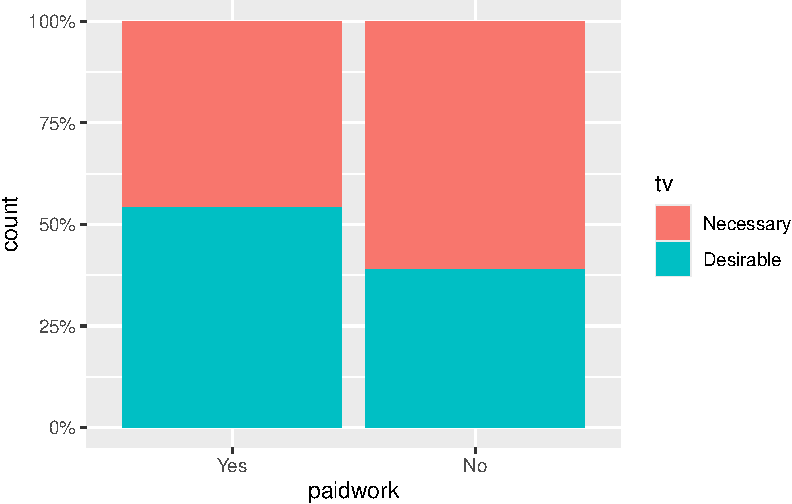
\includegraphics[keepaspectratio]{03_categorical_files/figure-pdf/unnamed-chunk-30-1.pdf}}

We can also build a \textbf{clustered bar chart} which we can create in
two different ways. The first is the classic clustered bar chart using
the option \textbf{position=``dodge'' (position=``dodge2'' will leave a
space between the bars)}

\begin{Shaded}
\begin{Highlighting}[]
\CommentTok{\# clustered bar chart}
\NormalTok{omni }\SpecialCharTok{|\textgreater{}} 
  \FunctionTok{drop\_na}\NormalTok{(tv, paidwork) }\SpecialCharTok{|\textgreater{}} 
  \FunctionTok{ggplot}\NormalTok{( }\FunctionTok{aes}\NormalTok{(}\AttributeTok{x=}\NormalTok{paidwork)) }\SpecialCharTok{+}
  \FunctionTok{geom\_bar}\NormalTok{(}\AttributeTok{stat=}\StringTok{"count"}\NormalTok{, }\FunctionTok{aes}\NormalTok{(}\AttributeTok{fill=}\NormalTok{tv), }
           \AttributeTok{position=}\StringTok{"dodge"}\NormalTok{) }
\end{Highlighting}
\end{Shaded}

\pandocbounded{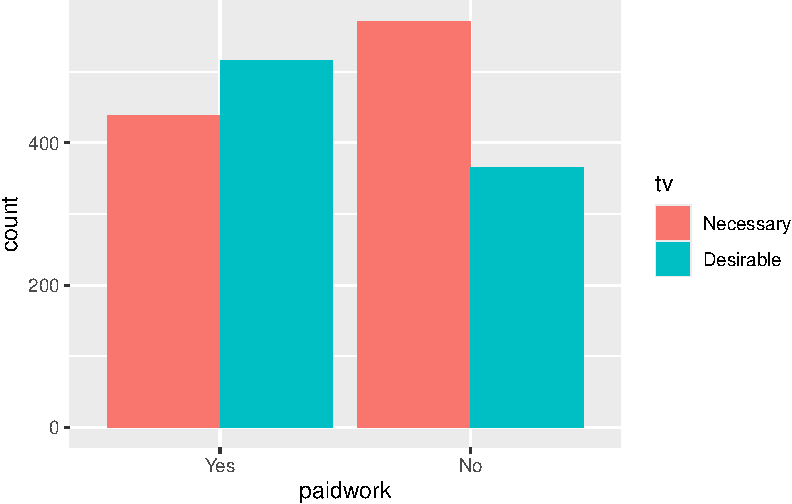
\includegraphics[keepaspectratio]{03_categorical_files/figure-pdf/unnamed-chunk-31-1.pdf}}

To add percentages to a clustered bar chart is a bit cumbersome but here
is a possible solution which basically involves calculating directly the
proportions before plotting them. It requires an additional package
called \textbf{ggstats} for geom\_bar() to recognise proportions as the
quantity to plot

\begin{Shaded}
\begin{Highlighting}[]
\NormalTok{omni }\SpecialCharTok{|\textgreater{}} 
  \FunctionTok{drop\_na}\NormalTok{(tv, paidwork) }\SpecialCharTok{|\textgreater{}} 
  \FunctionTok{group\_by}\NormalTok{ (paidwork, tv) }\SpecialCharTok{|\textgreater{}}
  \FunctionTok{count}\NormalTok{() }\SpecialCharTok{|\textgreater{}} 
  \FunctionTok{ggplot}\NormalTok{(}\FunctionTok{aes}\NormalTok{(}\AttributeTok{x=}\NormalTok{paidwork, }\AttributeTok{fill =}\NormalTok{ tv, }\AttributeTok{weight =}\NormalTok{ n, }
              \AttributeTok{by =}\NormalTok{ tv, }\AttributeTok{y =} \FunctionTok{after\_stat}\NormalTok{(prop))) }\SpecialCharTok{+}
  \FunctionTok{geom\_bar}\NormalTok{(}\AttributeTok{stat=}\StringTok{"prop"}\NormalTok{, }
           \AttributeTok{position=}\StringTok{"dodge"}\NormalTok{) }\SpecialCharTok{+}
  \FunctionTok{scale\_y\_continuous}\NormalTok{(}\AttributeTok{labels =}\NormalTok{ scales}\SpecialCharTok{::}\NormalTok{percent)}
\end{Highlighting}
\end{Shaded}

\pandocbounded{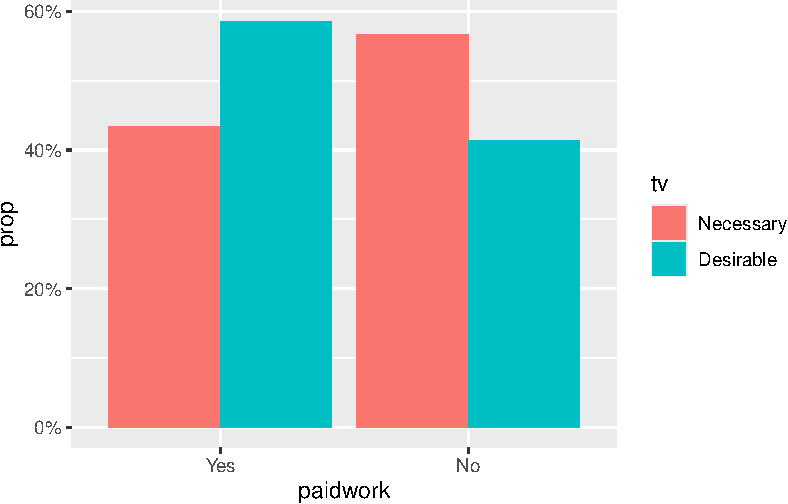
\includegraphics[keepaspectratio]{03_categorical_files/figure-pdf/unnamed-chunk-32-1.pdf}}

Rather than clustering within the same graph, an alternative is to use
faceting:

\begin{Shaded}
\begin{Highlighting}[]
\CommentTok{\# "faceted" clustered bar chart}
\NormalTok{omni }\SpecialCharTok{|\textgreater{}} 
  \FunctionTok{drop\_na}\NormalTok{(tv, paidwork) }\SpecialCharTok{|\textgreater{}} 
  \FunctionTok{ggplot}\NormalTok{(}\FunctionTok{aes}\NormalTok{(}\AttributeTok{x=}\NormalTok{tv)) }\SpecialCharTok{+}
  \FunctionTok{geom\_bar}\NormalTok{(}\AttributeTok{stat=}\StringTok{"count"}\NormalTok{) }\SpecialCharTok{+} 
  \FunctionTok{facet\_wrap}\NormalTok{(}\SpecialCharTok{\textasciitilde{}}\NormalTok{paidwork)}
\end{Highlighting}
\end{Shaded}

\pandocbounded{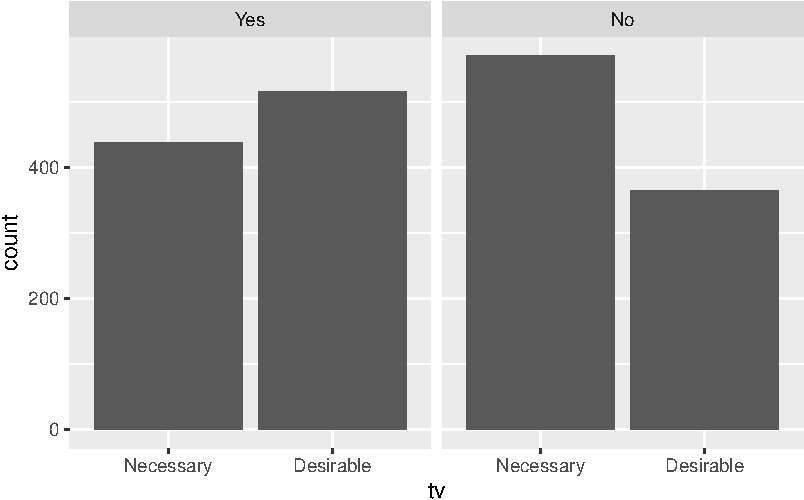
\includegraphics[keepaspectratio]{03_categorical_files/figure-pdf/unnamed-chunk-33-1.pdf}}

And we can obviously add labels and titles using the same functions as
before.

\section{Exercise II}\label{exercise-ii}

Write the code to produce the contingency table and clustered and
stacked bar charts below. Describe the bivariate distribution of item
``appropriate clothes for a job interview'' (variable \emph{jobfrock})
across the educational categories of variable \emph{graduate}.

\begin{verbatim}

    Graduates Not Graduates 
          347          1582 
\end{verbatim}

\begin{verbatim}

Necessary Desirable 
     1236       643 
\end{verbatim}

\begin{verbatim}
               
                Necessary Desirable
  Graduates         71.39     28.61
  Not Graduates     64.46     35.54
\end{verbatim}

\pandocbounded{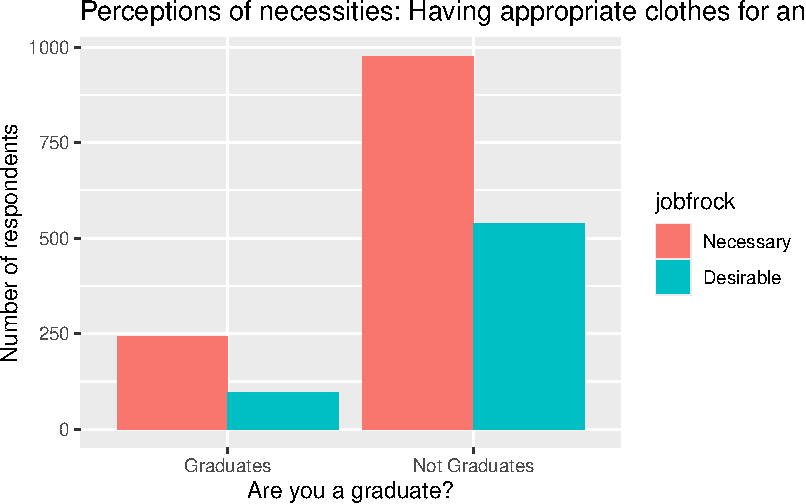
\includegraphics[keepaspectratio]{03_categorical_files/figure-pdf/unnamed-chunk-34-1.pdf}}

\pandocbounded{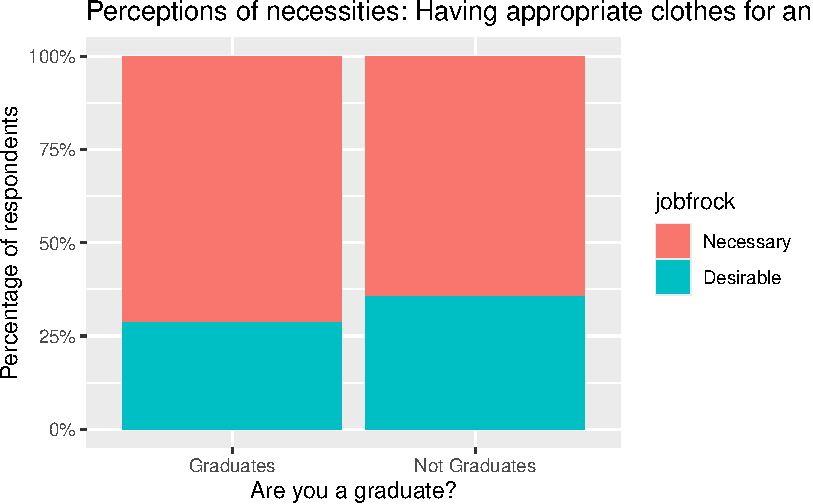
\includegraphics[keepaspectratio]{03_categorical_files/figure-pdf/unnamed-chunk-34-2.pdf}}

\bookmarksetup{startatroot}

\chapter{Cleaning and preparing data}\label{cleaning-and-preparing-data}

\bookmarksetup{startatroot}

\chapter{Inference}\label{inference}

\section{}\label{section}

\section{whatveer wq}\label{whatveer-wq}

\bookmarksetup{startatroot}

\chapter{Summary}\label{summary}

In summary, this book has no content whatsoever.

\begin{Shaded}
\begin{Highlighting}[]
\DecValTok{1} \SpecialCharTok{+} \DecValTok{1}
\end{Highlighting}
\end{Shaded}

\begin{verbatim}
[1] 2
\end{verbatim}

\bookmarksetup{startatroot}

\chapter*{References}\label{references}
\addcontentsline{toc}{chapter}{References}

\markboth{References}{References}

\protect\phantomsection\label{refs}




\end{document}
